\chapter{Chapitre 6 : Détection des problèmes}

\noindent Ce chapitre propose un tour d'horizon concis, visuel et orienté code de la manière dont nous détectons les problèmes de qualité des données après l'appariement des arrêts ATLAS avec les nœuds OSM. Nous présentons les types de problèmes, expliquons pourquoi et comment nous les priorisons, montrons de brefs extraits des règles, et concluons par une réflexion et des pistes d'amélioration concrètes. Attendez-vous à de petits extraits de code, des graphes compacts et un modèle mental simple pour trier des milliers d'anomalies.

\section{Ce que nous détectons (types de problèmes)}
Notre pipeline signale les problèmes au niveau consolidé des \texttt{stops} et les enregistre dans une table normalisée \texttt{problems}. Quatre familles sont actuellement prises en charge :
\begin{itemize}
  \item \textbf{Problèmes de distance} — une paire ATLAS–OSM appariée est trop éloignée (en mètres).
  \item \textbf{Problèmes de non-appariement} — un arrêt existe dans un jeu de données (ATLAS ou OSM) sans pendant plausible à proximité.
  \item \textbf{Problèmes d'attributs} — conflits de métadonnées sur des paires appariées (opérateur, nom officiel, référence locale, UIC).
  \item \textbf{Doublons (informationnels)} — SLOIDs dupliqués côté ATLAS ou nœuds OSM dupliqués pour la même plateforme \texttt{(uic\_ref, local\_ref)} ; utiles à la revue mais pas contradictoires en soi.
\end{itemize}

Chaque problème détecté possède un \emph{type}, une \emph{solution} optionnelle (pouvant être renseignée plus tard via des « solutions persistantes »), et une \textbf{priorité} numérique (P1 la plus haute, P3 la plus basse) afin de concentrer l'effort.

\section{Pourquoi prioriser}
Les problèmes sont nombreux et n'ont pas tous la même urgence. Un écart de 120 m dans un pôle d'échanges très fréquenté peut être bien plus impactant qu'une légère différence de chaîne de caractères d'opérateur. Les règles de priorité capturent cette intuition pour que l'interface web fasse ressortir d'abord ce qui compte.

\section{Comment les priorités sont attribuées}
Nous calculons les priorités par famille de problèmes à l'aide de règles simples et interprétables. Ci-dessous, des extraits compacts qui reflètent la logique de production.

\subsection{Priorités pour la distance}
Intuition : de grands écarts spatiaux sont suspects ; nous sommes plus stricts pour les entrées opérées par les CFF (rail).

\begin{codebox}[language=Python]{Priorisation distance — \texttt{compute\_distance\_priority}}
# P1 : >80 m pour non-CFF
# P2 : 25--80 m pour non-CFF
# P3 : >25 m pour CFF OU 15--25 m pour tout operateur
def compute_distance_priority(record):
    d = float(record["distance_m"])
    is_sbb = (record["csv_business_org_abbr"].upper() == "SBB")
    if d > 80 and not is_sbb:
        return 1
    if 25 < d <= 80 and not is_sbb:
        return 2
    if d > 25 and is_sbb:
        return 3
    if 15 < d <= 25:
        return 3
    return None  # aucun probleme de distance
\end{codebox}

\noindent Ceci reflète le code dans \texttt{matching\_process/problem\_detection.py} et s'applique quand une paire est étiquetée \texttt{matched}.

\subsection{Priorités pour les non-appariements}
Intuition : être isolé sans pendant proche est plus sévère ; la distance absolue et la disponibilité UIC/plateformes aident à classer l'urgence.

\begin{codebox}[language=Python]{Règles — non-appariements ATLAS/OSM}
# Entree ATLAS uniquement
if nearest_osm_distance is None or nearest_osm_distance > 80:
    P1
elif nearest_osm_distance > 50:
    P2
elif uic_platform_counts_mismatch:
    P2
else:
    P3

# Noeud OSM uniquement
if atlas_count_for_same_uic == 0:
    P1
elif nearest_atlas_distance is None or nearest_atlas_distance > 50:
    P2
elif uic_platform_counts_mismatch:
    P2
else:
    P3
\end{codebox}

\noindent Les distances au plus proche voisin sont calculées avec un KD-tree sur des coordonnées de sphère unitaire (rapide et numériquement stable). Le rayon d'isolement utilisé ailleurs est de \texttt{50 m} :

\begin{codebox}[language=Python]{Calcul voisinage — KD-tree et rayon d'isolement}
ISOLATION_CHECK_RADIUS_M = 50
radius_rad = 2 * sin((radius_m / 6371000.0) / 2)
indices = kdtree.query_ball_point(unit_xyz(point), radius_rad)
is_isolated = (len(indices) == 0)
\end{codebox}

\subsection{Priorités pour les attributs}
Intuition : certains champs sont des identifiants (UIC, noms officiels) et pèsent davantage que des champs d'affichage ou opérationnels.

\begin{codebox}[language=Python]{Priorisation attributs — \texttt{compute\_attributes\_priority}}
# P1 : UIC different OU nom officiel different
# P2 : \texttt{local_ref} different
# P3 : operateur different
def compute_attributes_priority(record):
    if record["number"] != record["osm_uic_ref"]:
        return 1
    if lower(record["csv_designation_official"]) != lower(record["osm_uic_name"]):
        return 1
    if lower(record["csv_designation"]) != lower(record["osm_local_ref"]):
        return 2
    if lower(record["csv_business_org_abbr"]) != lower(record["osm_operator"]):
        return 3
    return None
\end{codebox}

\section{Ce que cela donne dans l'application web}
L'interface propose des filtres simples pour permettre une triage rapide :
\begin{itemize}
  \item \textbf{Filtrer par type de problème} : \texttt{distance}, \texttt{unmatched}, \texttt{attributes}, \texttt{duplicates}.
  \item \textbf{Filtrer par priorité} : \texttt{P1}, \texttt{P2}, \texttt{P3}.
  \item \textbf{Trier} : p. ex. distance la plus grande d'abord, ou par ordre alphabétique du nom d'arrêt.
\end{itemize}

\noindent Nous insérerons ici des captures d'écran de l'interface (filtres et listes de problèmes). Pour référence, les ressources existantes sont montrées ci-dessous et pourront être mises à jour ultérieurement :

\begin{figure}[h]
  \centering
  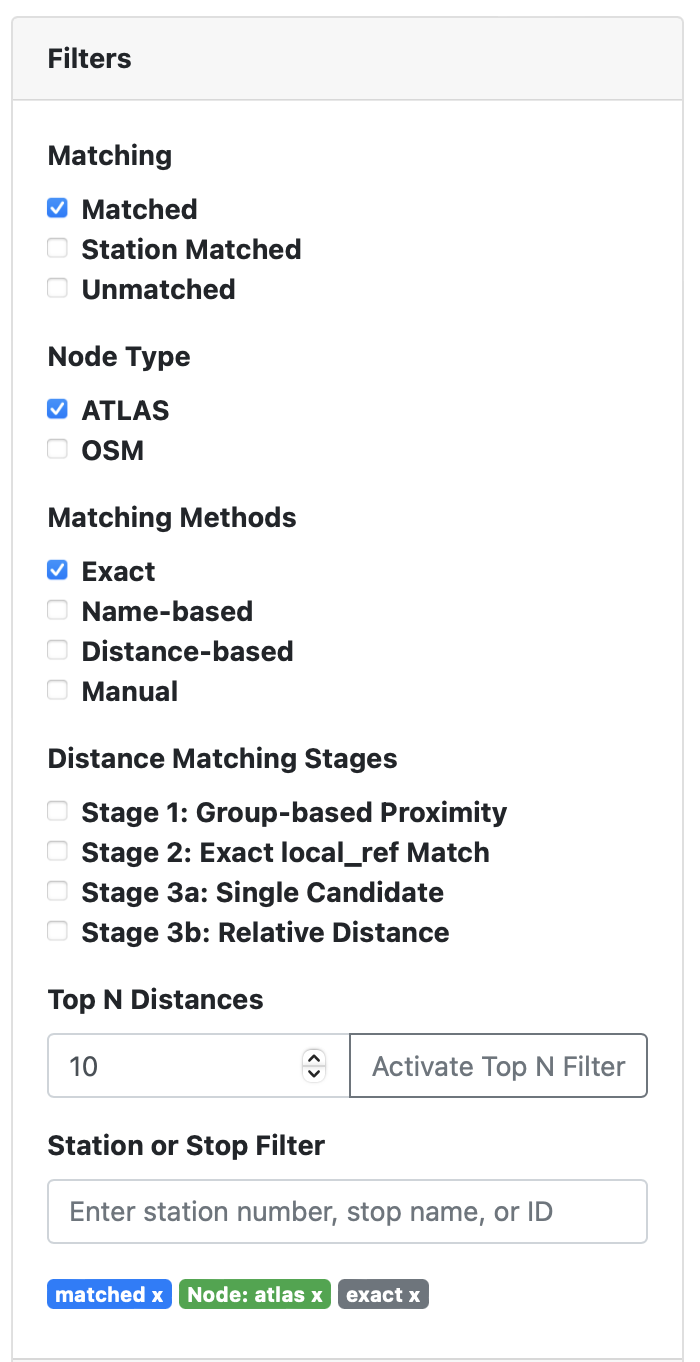
\includegraphics[width=0.85\textwidth]{../figures/webapp/filters.png}
  \caption{Filtres de l'application web : par type de problème et priorité.}
\end{figure}

\begin{figure}[h]
  \centering
  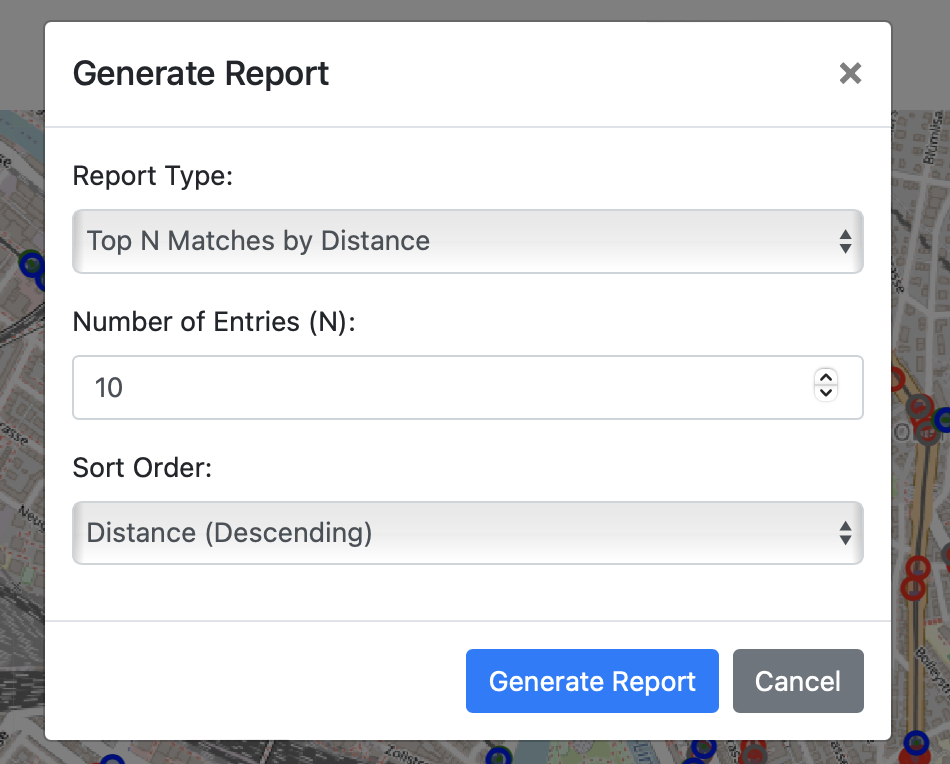
\includegraphics[width=0.85\textwidth]{../figures/webapp/report.png}
  \caption{Vue de rapport centrée sur les problèmes (esquisse).}
\end{figure}

\section{Chiffres de la dernière exécution}
Voici les compteurs de haut niveau affichés après l'import (pour traçabilité) :

\begin{center}
\small
\begin{tabular}{l r}
\toprule
Métrique & Nombre \\
\midrule
Total des arrêts importés & \textbf{77\,074} \\
Problèmes de distance & \textbf{11\,321} \\
Problèmes de non-appariement & \textbf{28\,546} \\
Problèmes d'attributs & \textbf{13\,865} \\
Entrées avec problèmes multiples & \textbf{5\,179} \\
Entrées saines (aucun problème) & \textbf{25\,839} \\
\midrule
Entrées avec au moins un problème (dérivé) & \textbf{51\,235} \\
\bottomrule
\end{tabular}
\end{center}

\noindent Pour rendre ce chapitre encore plus informatif la prochaine fois, nous étendrons l'importeur pour journaliser et exporter des ventilations supplémentaires. D'ici là, des espaces réservés indiquent des statistiques à renseigner lors de la prochaine exécution :

\begin{itemize}
  \item \textbf{Problèmes de distance par palier} : P1=\textbf{XX}, P2=\textbf{XX}, P3=\textbf{XX} ; distance médiane=\textbf{XX} m, p90=\textbf{XX} m.
  \item \textbf{Non-appariements (ATLAS vs OSM)} : ATLAS uniquement=\textbf{XX}, OSM uniquement=\textbf{XX} ; répartition P1/P2/P3=\textbf{XX/XX/XX}.
  \item \textbf{Problèmes d'attributs par champ} : UIC=\textbf{XX}, nom=\textbf{XX}, \texttt{local\_ref}=\textbf{XX}, opérateur=\textbf{XX}.
  \item \textbf{Opérateurs les plus concernés par la distance} : CFF=\textbf{XX}, TPG=\textbf{XX}, ZVV=\textbf{XX}, ...
  \item \textbf{Gares avec le plus de problèmes} : top-10 avec décomptes=\textbf{XX}.
  \item \textbf{Part des arrêts avec au moins un problème} : \textbf{XX\%} globalement ; par canton=\textbf{XX\%}/\textbf{XX\%}/\textbf{XX\%}.
\end{itemize}

\noindent Comme contexte visuel pour les distances, nous réutiliserons les distributions globales calculées précédemment (espaces réservés affichés ici ; seront mises à jour lors du prochain import) :

\begin{figure}[h]
  \centering
  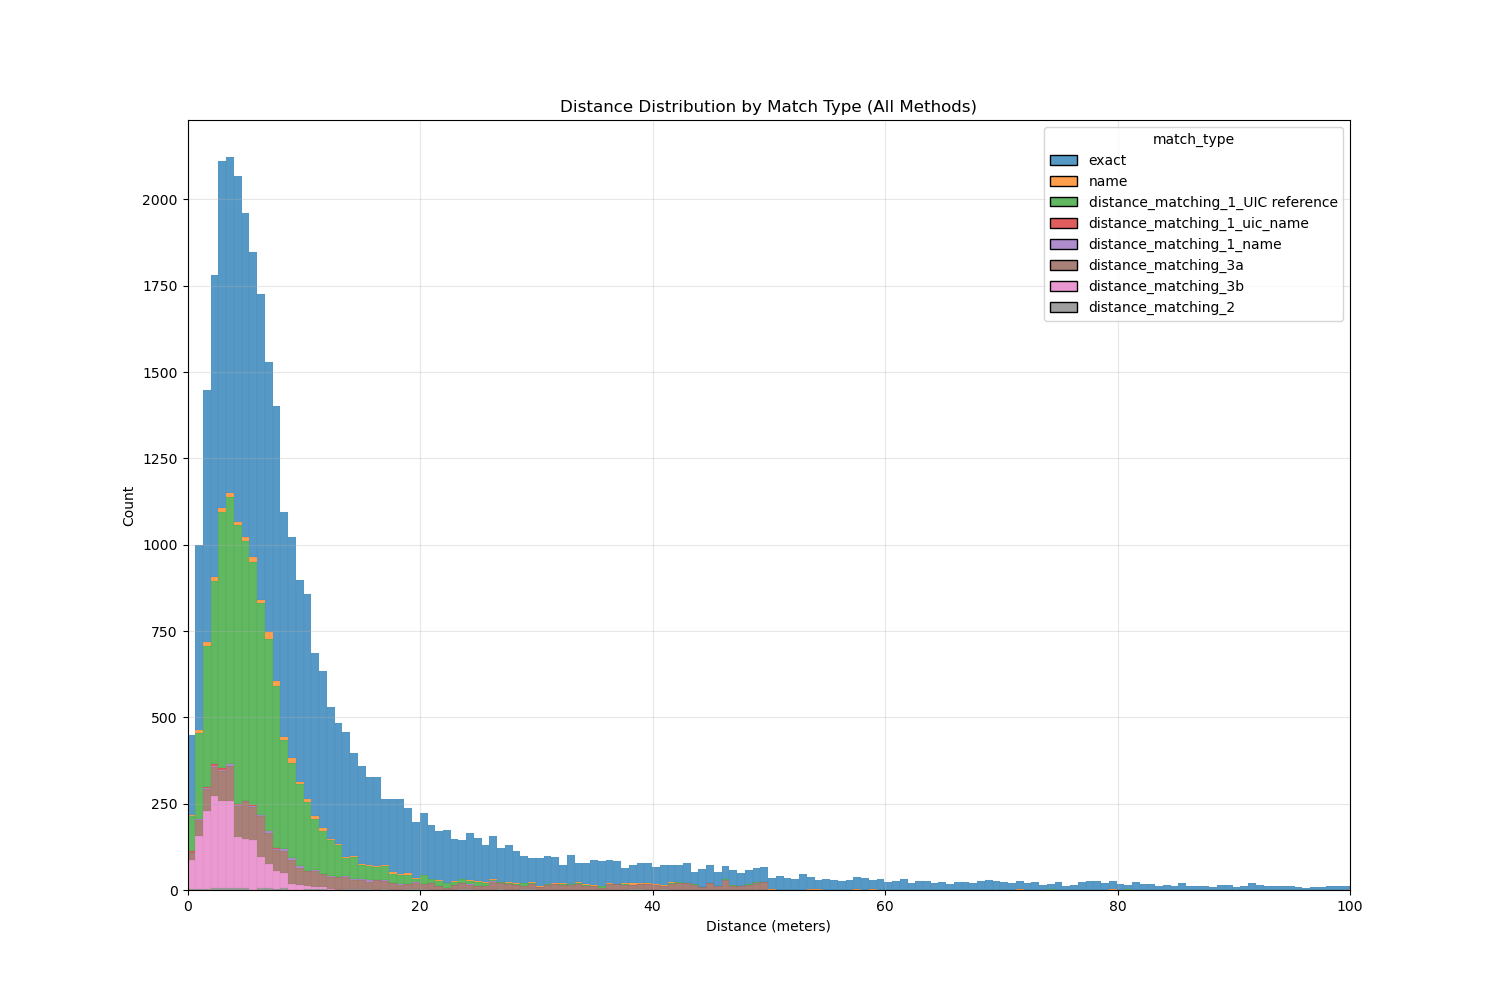
\includegraphics[width=0.75\textwidth]{../figures/plots/distance_distribution_all.png}
  \caption{Vue d'ensemble de la distribution des distances pour les paires appariées (illustratif).}
\end{figure}

\begin{figure}[h]
  \centering
  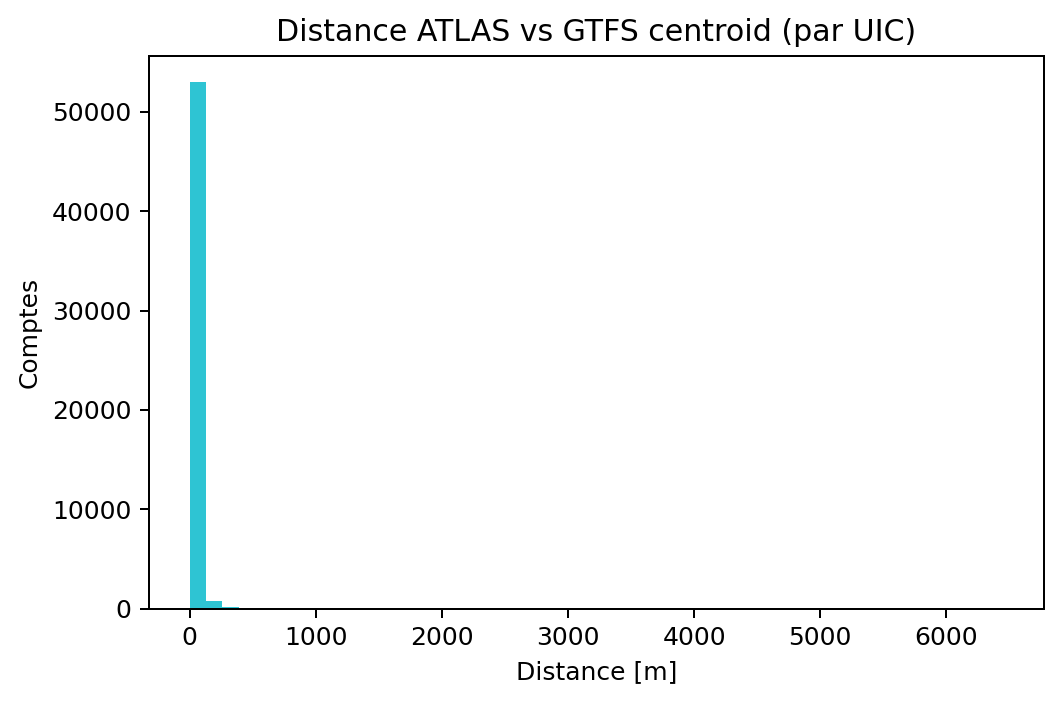
\includegraphics[width=0.75\textwidth]{../figures/plots/atlas_vs_gtfs_distance_hist.png}
  \caption{Exemple d'histogramme des distances (à aligner avec les seuils de problème).}
\end{figure}

\section{Persistance et flux de travail}
Deux mécanismes rendent la revue efficace dans le temps :
\begin{itemize}
  \item \textbf{Solutions persistantes} — une fois un problème résolu manuellement (p. ex. marqué \texttt{manual} pour un non-appariement), la décision est conservée et réappliquée lors des imports suivants.
  \item \textbf{Notes par côté} — les réviseurs peuvent ajouter des notes ATLAS/OSM qui persistent et s'affichent auprès de l'arrêt.
\end{itemize}

\noindent Cela est appliqué à la fin de l'import :
\begin{codebox}[language=Python]{Réapplication des solutions persistantes}
for ps in persistent_solutions:
    matching_stops = find_stops_by(sloid=ps.sloid, osm_node_id=ps.osm_node_id)
    for stop in matching_stops:
        problem = find_problem(stop, type=ps.problem_type)
        if problem:
            problem.solution = ps.solution
            problem.is_persistent = True
\end{codebox}

\section{Le modèle mental d'un réviseur}
En pratique, nous suggérons ce tri :
\begin{enumerate}
  \item Filtrer \textbf{distance / P1} et trier par distance décroissante. Corriger d'abord les erreurs flagrantes de géocodage.
  \item Puis \textbf{unmatched / P1}, en ciblant les cas sans pendant par UIC ou avec des écarts très importants.
  \item Traiter \textbf{attributes / P1}, notamment les divergences UIC/nom qui peuvent indiquer une mauvaise identité.
  \item Épurer les seaux P2/P3 restants par passes rapides ; ajouter des notes ou marquer comme cas limites acceptés si pertinent.
\end{enumerate}

\section{Réflexion et prochaines étapes}
\textbf{Ce qui fonctionne bien}. Les priorités sont simples et explicables ; les réviseurs peuvent se concentrer d'abord sur les problèmes les plus impactants. L'approche KD-tree rend les vérifications d'isolement rapides à l'échelle du pays, et les solutions persistantes éliminent les ressaisies d'une importation à l'autre.

\textbf{Pistes d'amélioration}.
\begin{itemize}
  \item \emph{Calibrage des seuils}. Apprendre des seuils à partir de données labellisées ou les adapter au contexte (urbain vs rural, bus vs rail).
  \item \emph{Vérifications spatiales enrichies}. Pour les grappes denses, compléter la distance point-à-point par des comparaisons de courts trajets ou des heuristiques de groupement de quais.
  \item \emph{Robustesse opérateur et dénominations}. Étendre la normalisation (diacritiques, abréviations) et tirer parti d'alias multilingues.
  \item \emph{Sémantique des doublons}. Ajouter un groupement plus malin pour distinguer les vrais doublons d'une multiplicité de quais attendue.
  \item \emph{Modèle de score}. Combiner les signaux (distance, lignes, noms, UIC) dans un classement appris pour les cas ambigus ; conserver les règles en repli.
  \item \emph{Meilleurs résumés}. Exporter les comptes par palier et les principaux contributeurs directement pendant l'import pour afficher des histogrammes et tableaux de bord à jour (les \textbf{XX} ci-dessus).
\end{itemize}

\noindent En résumé : cette couche de détection est déjà exploitable et scalable. Avec quelques améliorations ciblées, nous pouvons accélérer le tri, réduire le bruit et suivre les progrès avec des métriques plus riches.